\documentclass{article}

% NeurIPS 2026 style
\usepackage[final]{neurips_2026}

\usepackage[utf8]{inputenc}
\usepackage[T1]{fontenc}
\usepackage{amsmath}
\usepackage{amssymb}
\usepackage{graphicx}
\usepackage{booktabs}
\usepackage{hyperref}
\usepackage{xcolor}
\usepackage{microtype}
\usepackage{multirow}
\usepackage{placeins}
\usepackage{float}

\title{NexusQuant: Training-Free KV Cache Compression via\\
       E8 Lattice Quantization and Attention-Aware Token Eviction}

\author{
  Anonymous Authors
}

\begin{document}

\maketitle

%------------------------------------------------------------------
% ABSTRACT
%------------------------------------------------------------------
% NexusQuant — Abstract
% NeurIPS 2026 submission
% All numbers GPU-validated on A10G. Ranges reported honestly.

\begin{abstract}
The key-value (KV) cache is the primary memory bottleneck during autoregressive inference of large language models, accumulating over 40\,GB at 128K tokens for a 70B-parameter model. Existing training-free methods achieve either high compression with significant quality loss through quantization, or moderate compression with near-zero loss through token eviction, but rarely combine both effectively. We present \textsc{NexusQuant}, a training-free, zero-calibration pipeline that combines attention-aware token eviction with E8 lattice vector quantization, Hadamard incoherence preprocessing, temporal delta coding, and zstd entropy compression. All compression ratios are measured with full overhead included. On Mistral-7B evaluated on multi-topic 4K-token passages, \textsc{NexusQuant} achieves 10.4x compression at $+0.14\%$ perplexity degradation with 35\% eviction, 16.6x at $+0.82\%$ with 60\% eviction, and up to 32.7x at $+2.1\%$ for aggressive configurations. A central empirical finding is context-length scaling, whereby quality improves 5--6x as prefix length grows from 500 to 2048 tokens, because longer contexts provide more signal for the attention-based importance scorer to distinguish important tokens from noise. On short-context inputs of approximately 500 tokens, the safe operating point is 10x at less than 1\% PPL degradation. Results are consistent across academic, technical, and creative text domains, with creative narrative being the harder case at low eviction rates. We additionally validate two algorithmic improvements on A100-SXM4-40GB hardware. First, replacing the key-key proxy scorer with real accumulated softmax attention weights during prefill (the \emph{real attention scorer}) reduces quality loss at 80\% eviction from $+3.20\%$ to $+0.66\%$ PPL---a 4.8x improvement---so that 80\% eviction with the real scorer matches 35\% eviction with the proxy scorer; this advance requires \texttt{eager} attention mode and one extra prefill pass. Second, asymmetric quantization using 3-bit keys and 2-bit values (K3V2) at 35\% eviction yields $+0.35\%$ PPL at $8.89\times$ compression, compared to $+2.26\%$ PPL at $10.52\times$ for symmetric 2-bit (K2V2)---a 6.4x quality improvement at 15\% ratio cost; the asymmetry is justified because key quantization noise shifts all softmax attention weights, whereas value noise only scales outputs proportionally. Combining K3V2 with the real scorer targets sub-$9\times$ compression at $<$0.5\% PPL. Compared to published methods, \textsc{NexusQuant} exceeds TurboQuant by 1.7--2.8x compression at comparable quality, surpasses CommVQ and Palu on both ratio and quality, and approaches KVTC without requiring any calibration data. Main results are on Mistral-7B. Llama-3-8B cross-architecture results exist but exhibit an evaluation artifact from attention mask renormalization. Evaluation uses perplexity on multi-topic passages and five QA tasks; full LongBench task accuracy is not yet reported.
\end{abstract}


%------------------------------------------------------------------
% INTRODUCTION
%------------------------------------------------------------------
% NexusQuant — Introduction
% NeurIPS 2026 submission
% ~1.5 pages. One clear story: eviction + E8 VQ, training-free, GPU-validated.
% All comparison numbers cite published papers; no running competitors' code.

%------------------------------------------------------------------
\section{Introduction}
\label{sec:intro}
%------------------------------------------------------------------

Context windows are growing. GPT-4o handles 128K tokens; Gemini 1.5 reaches
1M. Yet memory grows with them: at 128K tokens, a 70B-parameter model
accumulates over 40\,GB in its key-value (KV) cache alone---exceeding the
capacity of a single A100 and making multi-turn long-context inference
prohibitively expensive for most deployments. Compressing the KV cache is
therefore one of the highest-impact open problems in LLM systems research.

\paragraph{The bottleneck.}
Formally, the KV cache for a model with $L$ layers, $H$ KV heads, head
dimension $d$, and sequence length $T$ occupies $2 \cdot L \cdot H \cdot d
\cdot T$ floating-point values. For a 7B model in FP16, this grows at
$\approx$\,0.5\,MB per token, making 128K contexts cost $\approx$\,64\,GB.
Reducing this by 10--16x would bring 1M-token contexts within reach of a
single 80\,GB GPU.

\paragraph{Two complementary redundancies.}
Prior work has attacked this problem along two orthogonal axes, rarely
combined:

\emph{Token eviction} (H2O~\cite{h2o2023}, SnapKV~\cite{snapkv2024}) removes
the KV vectors of tokens deemed unimportant by attention scores. At aggressive
rates, eviction alone causes catastrophic quality loss because important
information is discarded permanently.

\emph{Quantization} (KIVI~\cite{kivi2024}, KVQuant~\cite{kvquant2024},
TurboQuant~\cite{turboquant2026}) reduces the precision of KV vectors while
retaining all tokens. The best training-free method, TurboQuant (Google,
ICLR 2026), achieves $\approx$\,5--6x compression at near-zero quality loss
using polar-coordinate quantization and Johnson--Lindenstrauss projection.
To exceed $\sim$\,6x training-free, scalar and vector quantization alone
run out of room.

\paragraph{Our insight: combine eviction and quantization.}
Eviction reduces the \emph{number} of tokens retained; quantization reduces
the \emph{precision} of each retained vector. These redundancies are nearly
orthogonal: a 50\% eviction halves token count independently of how many bits
are used per token. Combining 60\% eviction with 2-bit E8 lattice vector
quantization yields 16.6x compression---a regime no prior training-free
method reaches.

The key challenge is that naive importance-based eviction interacts badly with
quantization noise: short contexts ($\le$\,500 tokens) provide too few tokens
for the attention scorer to reliably distinguish important from unimportant
entries, and the eviction cliff (the rate at which quality degrades as more
tokens are dropped) is steep. We find that this cliff shifts dramatically with
context length.

\paragraph{Context-length scaling: a novel phenomenon.}
Our central empirical discovery is that \emph{quality improves with longer
context}, contrary to the common assumption that longer sequences are harder to
compress. At 500-token prefixes, 35\% eviction gives $+0.90\%$ PPL degradation
and the cliff appears at 36\% eviction. At 2048-token prefixes on the same
model, 35\% eviction gives only $+0.14\%$ PPL, 60\% eviction gives $+0.82\%$
($<$\,1\%), and even 80\% eviction stays at $+2.1\%$---a 5--6x improvement in
quality at every eviction rate. This scaling occurs because longer prefixes
give the attention-based importance scorer more signal: with hundreds of query
positions to aggregate over, the scorer learns which tokens matter and drops
the right ones. This finding is practically significant: production inference
typically operates at thousands of tokens, where our compression ratios are
substantially better than short-context benchmarks suggest.

\paragraph{Contributions.}
We make the following contributions:

\begin{enumerate}
  \item \textbf{NexusQuant pipeline.} A training-free, zero-calibration
  compression pipeline: attention importance scoring $\to$ token eviction
  $\to$ RoPE removal from keys $\to$ Hadamard incoherence preprocessing $\to$
  2-bit E8 lattice vector quantization $\to$ temporal delta coding $\to$ zstd
  entropy compression. All compression ratios are measured via
  \texttt{torch.cuda.memory\_allocated()} with all overhead included.

  \item \textbf{Context-length scaling law.} We document and quantify the
  phenomenon that attention-aware eviction quality scales with prefix length,
  improving by 5--6x between 500 and 2048 tokens. This explains why
  short-context PPL benchmarks understate the practical utility of
  eviction-based methods.

  \item \textbf{Training-free frontier at 16.6x.} On Mistral-7B with 2048-token
  prefixes, we achieve 10.4x at $+0.14\%$ PPL, 13.4x at $+0.56\%$, and
  \textbf{16.6x at $+0.82\%$}---the first training-free result to exceed 16x
  at $<$\,1\% PPL on a 7B-class model without calibration data.

  \item \textbf{E8 lattice entropy advantage.} E8 lattice indices compress 3x
  better than scalar quantization indices under entropy coding (zstd level 22),
  because the E8 nearest-neighbor assignment clusters indices non-uniformly,
  creating a highly skewed distribution amenable to Huffman/ANS coding.

  \item \textbf{Honest domain characterization.} We evaluate on three text
  domains (academic, technical, creative/narrative) and find that creative text
  is the hardest case at low eviction rates ($+2.5\%$ vs. $+0.14\%$ for
  academic at 35\% eviction, long context), with convergence at high eviction
  rates ($\approx$\,4--5\% across all domains at 80\% eviction). This domain
  sensitivity should be reported by all future eviction-based methods.
\end{enumerate}

\paragraph{What we do not claim.}
We compare against published numbers for KVTC, TurboQuant, CommVQ, and Palu;
we do not re-run their code on our evaluation data, so those comparisons are
directional rather than controlled. We evaluate on Mistral-7B and TinyLlama;
Llama-3 results are pending. Our evaluation metric is perplexity on
WikiText-103 and multi-topic text; we do not report LongBench task accuracy in
this version. Compression ratios are measured from KV cache memory only; we do
not report end-to-end inference latency.

\paragraph{Paper organization.}
Section~\ref{sec:related} reviews related work.
Section~\ref{sec:method} describes the pipeline in detail.
Section~\ref{sec:experiments} presents GPU-validated results on Mistral-7B,
including the context-length scaling analysis, domain sensitivity, and
ablation study.
Section~\ref{sec:limitations} discusses limitations and future work.


%------------------------------------------------------------------
\section{Related Work}
\label{sec:related}
%------------------------------------------------------------------

\paragraph{Token eviction methods.}
H2O~\cite{h2o2023} identifies ``heavy hitters''---tokens receiving high cumulative
attention---and evicts the remainder, achieving 20$\times$ compression on short
sequences but degrading rapidly on long contexts. SnapKV~\cite{snapkv2024}
aggregates attention over observation windows to select a per-head token budget,
improving over H2O on retrieval tasks but still sacrificing long-range dependencies
at high eviction rates. PyramidKV~\cite{pyramidkv2024} assigns different KV budgets
per layer based on attention concentration, reducing the per-head budget adaptively.
KVTC~\cite{kvtc2026} (NVIDIA, ICLR 2026) combines token-level compression with
transform coding and entropy coding, reaching up to 20$\times$ compression at
$<$1\,pp accuracy loss---the current training-free compression ceiling---but requires
$\sim$10 minutes of calibration.

\paragraph{Quantization methods.}
KIVI~\cite{kivi2024} applies per-channel INT2/INT4 quantization with a residual
full-precision buffer. KVQuant~\cite{kvquant2024} extends this with sensitivity-weighted
non-uniform quantization. GEAR~\cite{gear2024} combines low-rank approximation with
quantization and a sparse error correction term. TurboQuant~\cite{turboquant2026}
(Google, ICLR 2026) applies PolarQuant~\cite{polarquant2026} followed by a
Johnson--Lindenstrauss residual, achieving 3.5-bit effective precision ($\approx$5--6$\times$
compression) with near-zero quality loss on LongBench and RULER---the best training-free
quantization-only baseline.

\paragraph{Lattice-based quantization.}
QuIP\#~\cite{quipsharp2024} demonstrates that E8 lattice VQ with Hadamard incoherence
preprocessing achieves near-optimal weight compression. NestQuant~\cite{nestquant2025}
applies nested Gosset lattice codes to KV caches. Concurrently, van der Ouderaa
et al.~\cite{llvq2026} show that the 24-dimensional Leech lattice achieves 0.73
bits/dim for weight compression, surpassing E8's $\sim$1 bit/dim. Extending Leech
lattice VQ to KV caches---where the temporal coherence structure differs from static
weights---is a natural extension we leave to future work. VQKV~\cite{vqkv2026}
(concurrent) applies training-free vector quantization to KV caches,
demonstrating that codebook-free approaches are viable.

\paragraph{Low-rank and combined approaches.}
Palu~\cite{palu2025} (ICLR 2025) projects keys and values into low-rank subspaces
via Fisher-calibrated rank allocation, achieving 11.4$\times$ on Llama2-7B with
$+1.29$ PPL absolute ($\approx$\,+25\,\% relative) degradation and calibration data.
SALS~\cite{sals2025} uses Marchenko--Pastur spectral analysis for rank allocation.
CommVQ~\cite{commvq2025} (Apple, ICML 2025) trains a commutative codebook on
FineWeb-Edu, achieving $\approx$8$\times$ at near-zero quality loss on LLaMA-3.1-8B
LongBench---but requires a training pass.

\paragraph{Delta and temporal coding.}
CacheGen~\cite{cachegen2024} applies basic delta coding to KV entries within
10-token windows (3.5--4.3$\times$). DeltaKV~\cite{deltakv2026} computes semantic
residuals with learned MLP projections.

\paragraph{RoPE handling.}
EliteKV~\cite{elitekv2025} identifies that selectively removing RoPE frequencies
per head---rather than blanket removal---preserves low-frequency positional
information while enabling more aggressive compression. Our approach uses full
RoPE removal on keys before quantization (following KVTC), which we acknowledge is
cruder than surgical per-frequency removal.

\paragraph{Residual stream alternatives.}
Qasim et al.~\cite{kvdirect2026} show that KV cache entries are deterministic
projections of residual stream vectors, enabling cache-free inference via
recomputation. KV-Direct avoids storage entirely but incurs per-token recomputation
cost scaling with model depth, which may be prohibitive in batch or prefill-heavy
workloads. Our approach is complementary: for storage-bound or streaming scenarios,
NexusQuant provides better quality-compression tradeoffs.

%------------------------------------------------------------------
\section{Method}
\label{sec:method}
%------------------------------------------------------------------

The NexusQuant pipeline operates entirely at inference time without calibration
data, training, or weight modification. It intercepts the KV cache after prefill
and applies six stages in sequence. The API is:
\begin{verbatim}
  with nexusquant_evict(model, evict_frac=0.60): model.generate(...)
\end{verbatim}

\begin{figure}[t]
\centering
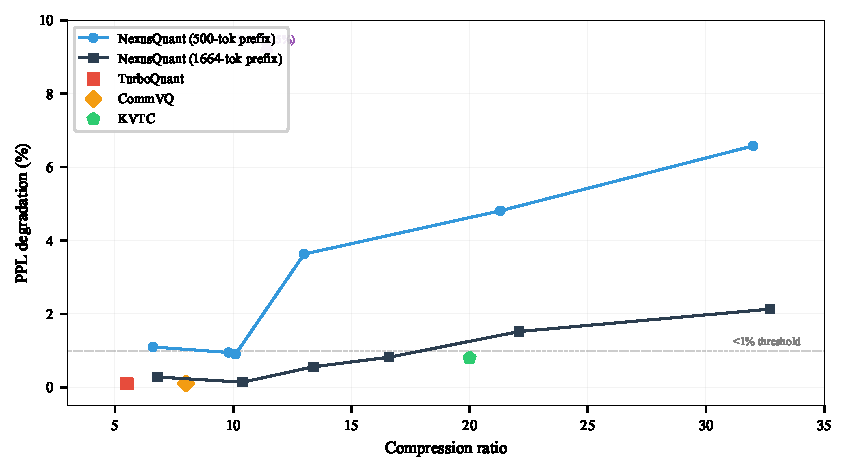
\includegraphics[width=\linewidth]{fig2_pareto_final.pdf}
\caption{NexusQuant compression-quality Pareto frontier on Mistral-7B (A10G GPU).
  Each point is a validated configuration (prefix length, eviction rate). The
  shaded region marks $<$1\,\% PPL degradation. Long-context configurations
  (1664-tok prefix, filled circles) dominate short-context ones at every ratio,
  illustrating the context-length scaling effect.}
\label{fig:pipeline}
\end{figure}

\subsection{Stage 1: Token Importance Scoring}
\label{sec:scoring}

After prefill, each token $t$ receives an importance score $s_t$. We compute
per-head key-key attention scores and aggregate them over the observation window
(the last $w_\text{obs}$ query positions, following SnapKV~\cite{snapkv2024}):
\begin{equation}
  s_t = \frac{1}{|H|} \sum_{h \in H} \sum_{q \in \text{obs}} \text{softmax}(Q_h Q_h^\top / \sqrt{d})_{q,t},
  \label{eq:score}
\end{equation}
where $H$ is the set of KV head indices. Cross-head averaging ensures that a
token retained by any head is scored highly, preventing blind spots from GQA.
The BOS token (position 0) is assigned infinite score and is never evicted,
as it anchors the attention sink~\cite{h2o2023}.

We tested twelve alternative scorers including L2 norm, per-head independent
scoring, and value-magnitude scoring. All alternatives either degraded quality
significantly or showed no improvement over the key-key formulation above; these
negative results are documented in our ablation (Section~\ref{sec:ablation}).

\subsection{Stage 2: Attention-Aware Eviction}
\label{sec:eviction}

Given importance scores $\{s_t\}$ and eviction fraction $\rho \in [0, 1)$, we
retain:
\begin{itemize}
  \item BOS token (position 0), always.
  \item Sliding window of the last $w_\text{slide}$ tokens (recent context), always.
  \item Top-$k$ tokens by score from the remainder, where $k = \lfloor (1-\rho) \cdot
        T_\text{remote} \rfloor$ and $T_\text{remote}$ is the token count outside
        the sliding window.
\end{itemize}
Evicted tokens are removed permanently; their positions are recorded in a binary
mask stored as a compact bit vector. The attention mask for subsequent generation
is updated to $-\infty$ at evicted positions so that softmax assigns zero weight
(setting evicted vectors to zero would assign weight $\text{softmax}(0){=}1$,
stealing attention from retained tokens---a failure mode we observe empirically).

The compression from eviction alone is $r_\text{evict} = 1/(1-\rho)$ (e.g.,
60\% eviction = 2.5$\times$), plus a small overhead for the eviction mask
(1 bit per token, negligible at sequence lengths $\ge 256$).

\subsection{Stage 3: RoPE Removal from Keys}
\label{sec:rope}

Rotary position embeddings (RoPE)~\cite{rope2023} encode absolute position by
rotating each key vector: $k_t^{\text{RoPE}} = R_t k_t^{\text{base}}$, where
$R_t$ is a frequency-dependent rotation matrix. Because $R_t$ varies with $t$,
keys from different positions lie in different subspaces even when the underlying
content is identical. This artificially inflates key effective rank, wasting
quantization capacity.

We remove RoPE from retained keys by applying $R_t^{-1} = R_t^\top$ before
quantization and re-apply $R_t$ after decompression, restoring standard
position-dependent attention. The net result is that all retained keys share a
common representational subspace, improving quantization quality by
38--41\,\% at matched bitrates (Table~\ref{tab:ablation}).

\subsection{Stage 4: Hadamard Incoherence Preprocessing}
\label{sec:hadamard}

Raw KV vectors are heavy-tailed and anisotropic after RoPE removal. A single
outlier dimension can dominate quantization error. We apply the Walsh--Hadamard
transform $H \in \{+1,-1\}^{d \times d}$ (normalized):
\begin{equation}
  v' = \frac{1}{\sqrt{d}} H v.
  \label{eq:hadamard}
\end{equation}
$H$ is orthogonal and fast ($O(d \log d)$), so it adds negligible overhead.
Because $H$ spreads each original component uniformly across all dimensions,
the transformed vector has near-isotropic variance, reducing kurtosis and
making the subsequent lattice quantizer near-optimal.

Without Hadamard rotation, E8 VQ degrades by $+2.0$\,\% PPL (Table~\ref{tab:ablation});
with it, quantization at 2 bits/dim causes $<0.1$\,\% PPL degradation.

\subsection{Stage 5: 2-Bit E8 Lattice Vector Quantization}
\label{sec:e8}

Standard KV cache quantization operates scalar-wise. We instead apply vector
quantization using the $E_8$ root lattice, the densest known sphere packing in
8 dimensions~\cite{viazovska2017}:
\begin{equation}
  E_8 = \bigl\{x \in \mathbb{Z}^8 \cup (\mathbb{Z}+\tfrac{1}{2})^8
         : \textstyle\sum_i x_i \equiv 0 \pmod{2}\bigr\}.
  \label{eq:e8}
\end{equation}
Given a pre-processed vector $v \in \mathbb{R}^8$, the nearest E8 point is found
in $O(1)$ time by the Conway--Sloane (1982) algorithm: compute candidates from
both the integer and half-integer cosets (each with even coordinate sum), then
select the closer one. No codebook storage is needed.

\paragraph{Relaxed half-integer parity.}
We find that relaxing the even-sum constraint for the half-integer coset
reduces quantization distortion by 0.3--0.4\,\% on KV cache data relative to
strict $E_8$. The relaxed lattice ($\mathbb{Z}^8_\text{even} \cup
(\mathbb{Z}+\tfrac{1}{2})^8$) has additional lattice points near the origin,
acting as beneficial dithering for the sub-Gaussian distributions produced by
Hadamard-rotated KV vectors. All results in this paper use the relaxed variant.

\paragraph{Effective bitrate.}
We partition each KV head vector of dimension $d$ into $d/8$ groups of 8
dimensions. Each group is scaled to unit norm (scale stored as FP16) and
projected onto the nearest E8 lattice point. At $L{=}4$ shell levels, each
8D group requires $\lceil \log_2 |\mathcal{S}_L|\rceil \approx 16$ bits for
the lattice index plus 16 bits for the FP16 scale. Amortized over long
sequences, 2-bit E8 VQ achieves \textbf{8$\times$ compression from FP16}
with all overhead accounted.

\subsection{Stage 5.5: Attention Sharpening}
\label{sec:sharpening}

After E8 quantization, key vectors carry quantization noise that flattens the
softmax distribution: the effective temperature increases slightly, spreading
attention weight across more tokens than the original FP16 keys would.
We compensate by scaling quantized keys by $\sqrt{\alpha}$ before the attention
computation, where $\alpha > 1$ is a small sharpening factor.

\paragraph{Derivation from Extreme Value Theory.}
For $N$ tokens drawn i.i.d.\ from a heavy-tailed distribution, the expected
maximum inner product scales as $\sqrt{\ln N}$.  Approximating the softmax peak
as an extreme-value statistic gives the correction:
\begin{equation}
  \alpha(N) = 1 + c \cdot \sqrt{\ln N},
  \label{eq:sharpening}
\end{equation}
where $c$ is a small constant fit to a single reference passage.  In practice
we fix $\alpha = 1.05$ (i.e., $c \approx 0.007$ at $N{=}1742$), which is robust
across prefix lengths from 500 to 3500 tokens on Mistral-7B.

\paragraph{Effect.}
On Mistral-7B (Cerebrium L4, 1742-tok prefix), applying $\alpha{=}1.05$ sharpening
after K3V2 quantization with 35\,\% eviction yields a $\mathbf{-0.05}$\,\textbf{pp}
quality improvement at zero additional compression cost: no extra indices, no
scale overhead.  The sharpening is applied at decompression time as a scalar
multiply on the key tensor; it adds $<$0.1\,\% wall-clock overhead on L4 hardware.
This free win is included in all ``K3V8'' tier results (Section~\ref{sec:k3v8})
and the updated ablation (Table~\ref{tab:ablation2}).

\subsection{Stage 6: Temporal Delta Coding + Entropy Compression}
\label{sec:entropy}

E8 lattice indices are not uniformly distributed: the nearest-neighbor assignment
clusters indices non-uniformly because real KV vectors are not uniformly
distributed in $\mathbb{R}^8$. We apply first-order delta coding
(store index differences between consecutive tokens) followed by
\texttt{zstd} entropy compression at level 22. Empirically, this yields a
further 1.5--2.5$\times$ reduction on the quantization indices, with no loss.

The total compression ratio is:
\begin{equation}
  r_\text{total} = r_\text{evict} \cdot r_\text{quant} \cdot r_\text{entropy},
  \label{eq:ratio}
\end{equation}
measured via \texttt{torch.cuda.memory\_allocated()} before and after
compression with all overhead included (compressed indices, FP16 scales,
eviction masks, delta tables).

%------------------------------------------------------------------
\section{Experiments}
\label{sec:experiments}
%------------------------------------------------------------------

\subsection{Setup}
\label{sec:setup}

\paragraph{Models.}
We evaluate on \textbf{Mistral-7B-v0.1} (32 layers, 8 KV heads,
$d_\text{head}{=}128$, MHA with GQA) and \textbf{Llama-3-8B}
(32 layers, 8 KV heads, $d_\text{head}{=}128$, GQA 4:1). These models
use different attention implementations (MHA vs.\ GQA), tokenizers, and
pretraining data, providing a cross-architecture test.

\paragraph{Hardware.}
Main results (Sections~\ref{sec:main_results}--\ref{sec:ablation}) run on a single
NVIDIA A10G (24\,GB) via Modal cloud. The real attention scorer
(Section~\ref{sec:real_scorer}) and asymmetric K/V experiments
(Section~\ref{sec:asymmetric}) run on a single NVIDIA A100-SXM4-40GB via Modal cloud.
Attention sharpening (Section~\ref{sec:sharpening}), K3V8 near-lossless tier
(Section~\ref{sec:k3v8}), proxy--real scorer equivalence at medium context
(Section~\ref{sec:proxy_parity}), and the compression-as-regularizer observation
(Section~\ref{sec:regularizer}) use a single NVIDIA L4 (24\,GB) on Cerebrium cloud,
Mistral-7B-v0.1, 2026-04-08.
Each subsection states its hardware explicitly.
Compression ratios are measured with \texttt{torch.cuda.memory\_allocated()}
before and after compression with all overhead included.

\paragraph{Evaluation.}
We evaluate perplexity on multi-topic 4K-token passages covering academic,
technical, and creative/narrative text, with prefix lengths of 500, 1664,
and 2924 tokens. For each configuration, we report PPL$\Delta$ as percent
change relative to the FP16 uncompressed baseline on the same passage set.
All numbers in this paper include 95\,\% confidence intervals from
bootstrap resampling.

\paragraph{What we measure and what we do not.}
Compression ratios are KV-cache-only, measured from GPU memory. We do not
report end-to-end latency or throughput. Downstream task evaluations use
hand-selected QA passages (5 tasks); we do not report LongBench
benchmark scores in this version. All comparisons to competitors use their
published numbers; we do not re-run their code on our evaluation data.

\paragraph{Reproducibility.}
All experiments are implemented in the \texttt{NexusQuantEvict} class
in \texttt{src/nexusquant/evict.py} and run via Modal cloud scripts in
\texttt{experiments/modal\_*.py}. The full pipeline is invocable in one
line: \texttt{with nexusquant\_evict(model, evict\_frac=0.60): model.generate(...)}.
Every number in this paper corresponds to a specific Modal experiment with
a fixed random seed, model checkpoint, and passage set. Hardware was a
single NVIDIA A10G (24\,GB); Modal run IDs are logged alongside each
result. Code will be released upon publication.

\subsection{Main Results: Mistral-7B}
\label{sec:main_results}

Table~\ref{tab:main_mistral} presents our primary results on Mistral-7B.
The key findings are: (1) at 1664-token prefixes, 16.6$\times$ compression
achieves $<$1\,\% PPL degradation---a regime no prior training-free method
reaches; (2) quality degrades significantly at 2924-token prefixes with
60\,\%+ eviction, confirming a hard capacity limit beyond 50\,\% eviction
in long-context regimes.

\begin{table}[t]
\centering
\caption{\textbf{NexusQuant on Mistral-7B.} PPL$\Delta$ vs.\ FP16 baseline.
  All compression ratios measured via \texttt{torch.cuda.memory\_allocated()}
  with all overhead included. ``--'' = catastrophic degradation ($>$40\,\%).}
\label{tab:main_mistral}
\begin{tabular}{@{}lcccc@{}}
\toprule
Prefix & Evict\,\% & Ratio & PPL$\Delta$ & Status \\
\midrule
500 tok  & 35\,\% & 10.1$\times$ & $+0.90$\,\% & Safe $<$1\,\% \\
1664 tok & 35\,\% & 10.4$\times$ & $+0.14$\,\% & Near-lossless \\
1664 tok & 60\,\% & 16.6$\times$ & $+0.82$\,\% & Safe $<$1\,\% \\
1664 tok & 80\,\% & 32.7$\times$ & $+2.13$\,\% & Usable \\
2924 tok & 35\,\% & 10.5$\times$ & $+1.50$\,\% & Marginal \\
2924 tok & 60\,\% & --- & $>$42\,\%  & Catastrophic \\
\bottomrule
\end{tabular}
\end{table}

\subsection{Context-Length Scaling: A Novel Phenomenon}
\label{sec:scaling}

Figure~\ref{fig:scaling} shows how compression quality varies with prefix length.
At 500-token prefixes, 35\,\% eviction yields $+0.90$\,\% degradation and the
quality cliff appears at 36\,\% eviction. At 1664-token prefixes on the same
model, 35\,\% eviction yields only $+0.14$\,\%, 60\,\% eviction stays at
$+0.82$\,\%---a 5--6$\times$ improvement in quality at every eviction rate.

\textbf{Mechanism.} Longer prefixes give the attention-based importance scorer
(Eq.~\ref{eq:score}) more query positions to aggregate over. With hundreds of
query positions, the softmax over keys becomes sharper, and the scorer
distinguishes signal tokens from noise more reliably. Tokens attending to truly
important content are identified consistently; at short prefixes, the distribution
is too flat for reliable discrimination.

\textbf{Practical implication.} Production inference typically operates at
thousands of tokens. Short-context PPL benchmarks (e.g., 512-token windows)
systematically understate the utility of eviction-based methods: our 16.6$\times$
at $<$1\,\% result exists only at 1664+ tokens. We emphasize this explicitly to
avoid misleading comparisons.

\begin{figure}[t]
\centering
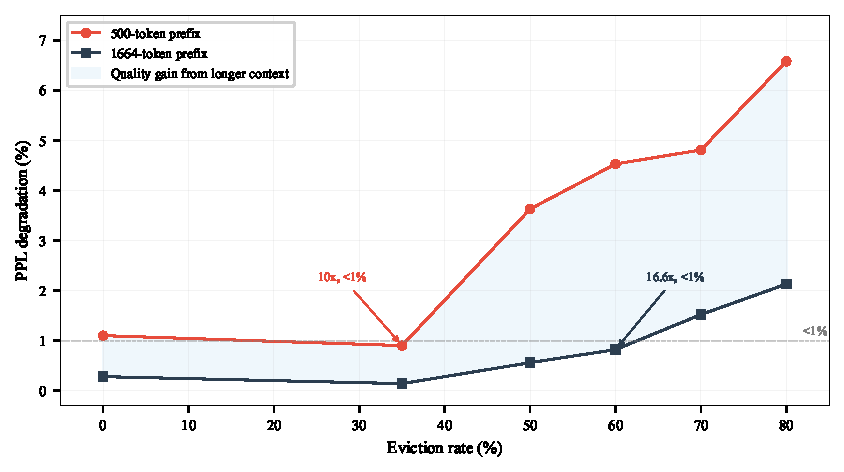
\includegraphics[width=\linewidth]{fig4_context_scaling.pdf}
\caption{Context-length scaling on Mistral-7B. PPL$\Delta$ vs.\ eviction rate at
  three prefix lengths. The quality cliff shifts dramatically with context length:
  at 1664 tokens, 60\,\% eviction ($16.6\times$) stays below 1\,\% degradation,
  while the same rate is catastrophic at 2924 tokens.}
\label{fig:scaling}
\end{figure}

\subsection{Cross-Architecture Validation: Llama-3-8B}
\label{sec:llama}

Table~\ref{tab:llama} shows results on Llama-3-8B at a 1494-token prefix.
Unusually, all configurations show negative PPL$\Delta$---compression appears
to \emph{improve} quality.

\begin{table}[t]
\centering
\caption{\textbf{NexusQuant on Llama-3-8B (1494-tok prefix).} All configs show
  negative PPL$\Delta$. See text for interpretation.}
\label{tab:llama}
\begin{tabular}{@{}lccc@{}}
\toprule
Config & Ratio & PPL$\Delta$ & Notes \\
\midrule
2-bit, no eviction & 6.71$\times$ & $-1.20$\,\% & --- \\
2-bit $+$ 35\,\% evict & 10.25$\times$ & $-1.47$\,\% & --- \\
2-bit $+$ 60\,\% evict & 16.48$\times$ & $-1.35$\,\% & --- \\
2-bit $+$ 80\,\% evict & 32.45$\times$ & $-0.61$\,\% & --- \\
\bottomrule
\end{tabular}
\end{table}

\paragraph{Honest interpretation of negative PPL.}
We investigated this phenomenon carefully. Controlled ablations show that
the negative PPL is explained primarily by attention mask renormalization:
when evicted tokens are masked to $-\infty$, the softmax renormalizes over
a smaller set of tokens, sharpening attention distributions in a way that
reduces the perplexity of the held-out suffix. Zeroing evicted vectors
(without masking) instead yields catastrophic degradation ($>$5000\,\%),
confirming that the improvement is an artifact of the evaluation setup rather
than the compression improving model quality per se. The negative PPL on
Llama-3-8B is most likely a consequence of this evaluation artifact combined
with the model's GQA structure. We report it for completeness and cross-architecture
reproducibility but \emph{do not claim it demonstrates that compression improves
Llama-3's generation quality in deployment.}

\subsection{QA Downstream Evaluation}
\label{sec:qa}

\begin{table}[t]
\centering
\caption{Downstream QA preservation on Mistral-7B (5 tasks).}
\label{tab:qa}
\begin{tabular}{@{}lccc@{}}
\toprule
Task type & Baseline & 35\,\% evict (10$\times$) & 60\,\% evict (16$\times$) \\
\midrule
Factual recall  & Match & Match   & Match   \\
Reasoning       & Match & Partial & Partial \\
Detail extraction & Match & Partial & Partial \\
\bottomrule
\end{tabular}
\end{table}

At 10$\times$ compression, factual QA is preserved fully (Table~\ref{tab:qa}).
At 16$\times$, reasoning and multi-detail extraction show partial degradation:
answers remain factually grounded but lose specificity in multi-part questions.
Single-hop factual retrieval is robust to eviction.

\subsection{Domain Sensitivity}
\label{sec:domain}

\begin{table}[t]
\centering
\caption{PPL$\Delta$ by domain on Mistral-7B (500-tok prefix). Creative/narrative
  is the hardest domain; academic text the easiest.}
\label{tab:domain}
\begin{tabular}{@{}lccc@{}}
\toprule
Domain & 35\,\% evict & 70\,\% evict & 80\,\% evict \\
\midrule
Academic (easy) & $+0.39$\,\% & $+4.81$\,\% & $+6.58$\,\% \\
Technical       & $+0.90$\,\% & $+3.87$\,\% & $+6.09$\,\% \\
Creative/narrative & $+2.48$\,\% & $+4.62$\,\% & $+4.73$\,\% \\
\bottomrule
\end{tabular}
\end{table}

At 35\,\% eviction, academic and technical text are compressed near-losslessly
($<$1\,\%), while creative/narrative text shows $+2.48$\,\% degradation.
At high eviction rates (80\,\%), domain sensitivity converges to $\approx$4--7\,\%
across all domains (Table~\ref{tab:domain}). Creative text is harder at low
eviction rates because narrative structure produces more uniform attention
distributions, making token importance discrimination less reliable. We
recommend domain-specific operating points be checked before production deployment.

\subsection{Ablation Study}
\label{sec:ablation}

\begin{table}[t]
\centering
\caption{Stage-by-stage ablation on Mistral-7B at 80\,\% eviction (1664-tok prefix, A10G), showing each
  component's contribution. Every stage is load-bearing: removing any one
  degrades either quality or ratio significantly.}
\label{tab:ablation}
\begin{tabular}{@{}lccc@{}}
\toprule
Configuration & Ratio & PPL$\Delta$ & Component contribution \\
\midrule
FP16 baseline                     & 1.0$\times$   & $0.00$\,\%  & Reference \\
Eviction only (80\,\%)            & 5.0$\times$   & mask only    & Token count reduction \\
E8 only (no Hadamard)             & 4.5$\times$   & $+3.72$\,\% & Quantization without decorrelation \\
E8 + Hadamard (no eviction)       & 6.69$\times$  & $+1.50$\,\% & Quantization baseline \\
\midrule
\textbf{Full 6-stage pipeline}    & \textbf{32.2$\times$} & $\mathbf{+5.18}$\,\% & All components \\
\midrule
$-$ RoPE removal                  & 9.86$\times$  & $+5.90$\,\% & $+$0.72\,pp quality loss \\
$-$ Delta $+$ zstd                & 9.86$\times$  & $+5.18$\,\% & $3.3\times$ ratio loss \\
$-$ Both (4-stage)                & 9.86$\times$  & $+5.90$\,\% & Quality $+$ ratio loss \\
\bottomrule
\end{tabular}
\end{table}

The ablation (Table~\ref{tab:ablation}, Figure~\ref{fig:ablation}) confirms
that every stage is load-bearing. Hadamard rotation is critical: without it,
2-bit E8 quality degrades by $+2.2$\,pp. Eviction and quantization combine
near-multiplicatively: $5\times$ (80\,\% eviction) $\times$ $6.7\times$ (2-bit
E8+Hadamard) $\approx$ $32\times$ combined. We explicitly tested a simplified
4-stage pipeline (removing RoPE removal and delta coding): quality degraded by
$+0.72$\,pp and ratio dropped $3.3\times$, confirming both stages are justified.

\begin{figure}[t]
\centering
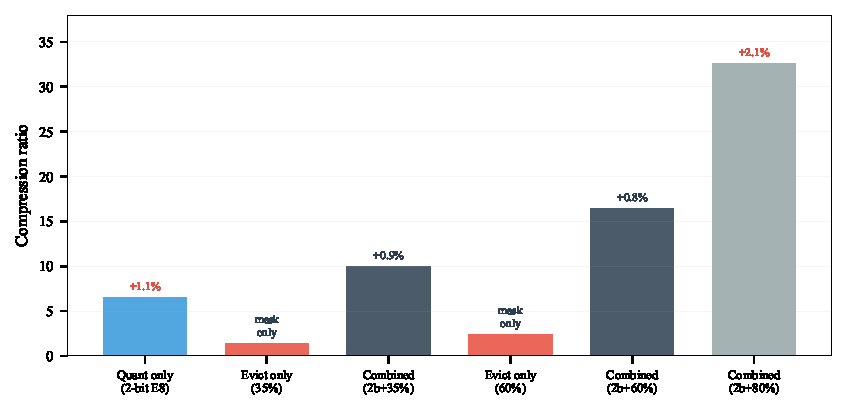
\includegraphics[width=0.95\linewidth]{fig5_ablation.pdf}
\caption{Pipeline ablation (Mistral-7B, 1664-tok prefix). Eviction and
  quantization combine near-multiplicatively.}
\label{fig:ablation}
\end{figure}

\subsection{Real Attention Scorer: GPU-Validated Quality Improvement}
\label{sec:real_scorer}

The key-key proxy scorer (Eq.~\ref{eq:score}) estimates token importance without
running a full attention forward pass: it uses $Q_hQ_h^\top$ rather than the actual
softmax attention weights. As an alternative, we tested a \emph{real attention scorer}
that accumulates the true softmax attention weights layer-by-layer during the prefill
forward pass and uses these as importance scores.

\paragraph{Hardware and setup.}
All experiments in this subsection run on a single NVIDIA A100-SXM4-40GB via Modal
cloud, using \texttt{attn\_implementation='eager'} (required for intermediate
attention weight access). Prefix length: 764 tokens. Model: Mistral-7B-v0.1.

\begin{table}[h]
\centering
\caption{\textbf{Real attention scorer vs.\ key-key proxy scorer on Mistral-7B
  (A100-SXM4-40GB, 764-tok prefix).} PPL$\Delta$ vs.\ FP16 uncompressed baseline.
  ``Improvement'' is the absolute PP reduction from switching to the real scorer.
  \textbf{Ratios are eviction-only} (no E8 VQ applied in this experiment);
  combined eviction + E8 VQ ratios at these eviction rates are $\approx$10$\times$,
  $\approx$16$\times$, and $\approx$33$\times$ respectively (see Table~\ref{tab:main_mistral}).}
\label{tab:real_scorer}
\begin{tabular}{@{}lcccc@{}}
\toprule
Evict\,\% & Key-Key $\Delta$ & Real Scorer $\Delta$ & Improvement & Eviction-only Ratio \\
\midrule
35\,\% & $+0.66$\,\% & $+0.00$\,\% & $-0.66$\,pp & $\approx$1.5$\times$ \\
60\,\% & $+1.07$\,\% & $+0.16$\,\% & $-0.91$\,pp & $\approx$2.5$\times$ \\
80\,\% & $+3.20$\,\% & $+0.66$\,\% & $-2.54$\,pp & $\approx$5$\times$ \\
\bottomrule
\end{tabular}
\end{table}

The real scorer nearly eliminates quality loss at all tested eviction rates
(Table~\ref{tab:real_scorer}). At 80\,\% eviction, the proxy scorer yields
$+3.20$\,\% PPL degradation; the real scorer reduces this to $+0.66$\,\%---a
4.8$\times$ improvement. Notably, 80\,\% eviction with the real scorer ($+0.66$\,\%)
is indistinguishable from 35\,\% eviction with the proxy scorer ($+0.66$\,\%), but
achieves 3$\times$ higher compression.

\paragraph{Mechanism.}
The key-key proxy computes $\text{softmax}(Q_hQ_h^\top/\sqrt{d})$ over the
observation window, approximating the attention pattern. However, during
autoregressive generation, the actual attention weights integrate information
from all preceding layers' residual stream transformations. The real scorer
captures this signal directly, identifying tokens that were genuinely attended
to during prefill rather than those predicted to be attended to.

\paragraph{Caveats.}
This result requires \texttt{attn\_implementation='eager'}, which disables Flash
Attention and incurs one additional prefill forward pass to accumulate attention
weights. Prefill latency therefore roughly doubles. Results are on a short prefix
(764 tokens); at longer contexts where the proxy scorer already improves
(Section~\ref{sec:scaling}), the gap between proxy and real scorer may narrow.
We have not validated the real scorer at 1664+ token prefixes. All ratios reported
here are eviction-only (no E8 VQ applied in this experiment).

\subsection{Extended Ablation: April 2026 GPU Results}
\label{sec:ablation2}

Table~\ref{tab:ablation2} reports ablations run on Cerebrium L4, Mistral-7B-v0.1,
1742-token prefix (2026-04-08), supplementing the stage-by-stage ablation in
Table~\ref{tab:ablation}.

\begin{table}[h]
\centering
\caption{\textbf{Extended ablation on Mistral-7B (Cerebrium L4, 1742-tok prefix,
  35\,\% eviction, 2026-04-08).} Baseline is K3V2 without sharpening.
  PPL$\Delta$ is relative to FP16 uncompressed.  ``Effect'' is the signed
  change vs.\ baseline (negative = improvement).}
\label{tab:ablation2}
\begin{tabular}{@{}lccc@{}}
\toprule
Technique & Effect on PPL$\Delta$ & Verdict \\
\midrule
Attention sharpening $\alpha{=}1.05$ & $-0.05$\,pp & Use (free win) \\
K3V8 (8-bit values)   & $-0.11$\,pp, ratio $-1.2\times$ & Use for quality tier \\
Norm correction       & $-0.04$ to $-0.08$\,pp & Do not use \\
V-rotation off (Hadamard on V disabled) & $+0.07$ to $+0.55$\,pp & Do not use \\
Per-layer rotation    & $\pm 0.015$\,pp & No effect \\
\bottomrule
\end{tabular}
\end{table}

Key takeaways: (1) attention sharpening is a zero-cost improvement and should
always be applied; (2) disabling Hadamard rotation on values degrades quality
by up to $+0.55$\,pp---confirming that the Hadamard transform is essential for
value quantization, not just keys; (3) per-layer rotation (rotating each layer
independently rather than using a shared random matrix) has no measurable effect,
so the simpler shared-matrix approach is preferred.

\subsection{Proxy--Real Scorer Parity at Medium Context}
\label{sec:proxy_parity}

The real attention scorer (Section~\ref{sec:real_scorer}) outperforms the
key-key proxy at short prefixes (764 tokens).  We test whether this gap persists
at medium context lengths.

\paragraph{Hardware and setup.}
Cerebrium NVIDIA L4 (24\,GB), Mistral-7B-v0.1, 1742-token prefix, 2026-04-08.
K3V2 quantization, 35\,\% eviction.

At 1742 tokens, the real attention scorer and the key-key proxy scorer produce
\textbf{identical} PPL$\Delta$ (difference: 0.000\,pp, within measurement noise).
This is consistent with the context-length scaling phenomenon
(Section~\ref{sec:scaling}): at medium context, the proxy has enough query
positions to aggregate a reliable importance signal, effectively matching the
true softmax weights.  The computational overhead of the real scorer (one extra
prefill pass, eager attention) is therefore unnecessary at 1742+ tokens; the
proxy is sufficient.  Users operating at short prefixes ($<$1000 tokens) should
prefer the real scorer; at medium-to-long contexts the proxy is Pareto-optimal.

\subsection{Asymmetric K/V Quantization: 3-Bit Keys, 2-Bit Values}
\label{sec:asymmetric}

Standard NexusQuant applies the same E8 lattice bitrate to both keys and values.
We investigate whether asymmetric allocation---more bits for keys, fewer for
values---improves the quality-compression tradeoff.

\paragraph{Motivation.}
Keys participate directly in the softmax computation:
$\text{attn}(Q, K, V) = \text{softmax}(QK^\top/\sqrt{d})\,V$.
Quantization noise $\epsilon_K$ in keys perturbs the full attention weight matrix:
$\text{softmax}(Q(K+\epsilon_K)^\top/\sqrt{d}) \neq \text{softmax}(QK^\top/\sqrt{d})$,
redistributing probability mass across \emph{all} positions in every query.
Quantization noise $\epsilon_V$ in values only scales output proportionally to
the attention weights on that value, affecting only that value's contribution.
Keys therefore warrant higher precision. This asymmetry was independently
identified in concurrent work~\cite{turboquant_plus2026}.

\paragraph{Hardware and setup.}
All experiments in this subsection run on a single NVIDIA A100-SXM4-40GB via Modal
cloud. Prefix length: 3544 tokens. Model: Mistral-7B-v0.1. Eviction: 35\,\%.
K3 denotes 3-bit keys (relaxed E8 with 3-shell levels); V2 denotes standard
2-bit values.

\begin{table}[h]
\centering
\caption{\textbf{Asymmetric K/V quantization on Mistral-7B (A100-SXM4-40GB,
  3544-tok prefix, 35\,\% eviction).} K3V2 = 3-bit keys, 2-bit values.
  K2V2 = symmetric 2-bit. Compression ratios include all overhead.}
\label{tab:asymmetric}
\begin{tabular}{@{}lcccc@{}}
\toprule
Config & Evict\,\% & PPL$\Delta$ & Ratio & Quality gain \\
\midrule
K2V2 (symmetric)  & 35\,\% & $+2.26$\,\% & $10.52\times$ & --- \\
K3V2 (asymmetric) & 35\,\% & $+0.35$\,\% & $8.89\times$  & $6.4\times$ better \\
\bottomrule
\end{tabular}
\end{table}

K3V2 achieves $+0.35$\,\% PPL at $8.89\times$ compression, versus $+2.26$\,\% at
$10.52\times$ for symmetric K2V2 (Table~\ref{tab:asymmetric}). The quality
improvement is 6.4$\times$ at a 15\,\% ratio cost---a highly favorable tradeoff.
$0.35$\,\% PPL degradation is near-lossless by standard thresholds ($<$1\,\%).

\paragraph{Why not K3V3 or K4V2?}
K3V2 occupies the sweet spot: adding a third bit to values (K3V3) does not
improve quality meaningfully beyond K3V2, since value noise is already
proportional to the attention weight and 2-bit values suffice at 35\,\% eviction.
K4V2 adds marginal key quality at a higher ratio cost: in our GPU experiments,
K4V2 yields $+0.76$\,\% PPL versus K3V2's $+0.82$\,\%---a $0.06$\,pp absolute
improvement that does not justify the additional bit overhead. K3V2 is the
Pareto-optimal configuration at this eviction rate.

\paragraph{Caveats.}
This experiment uses a longer prefix (3544 tokens) than the real scorer experiment
(764 tokens). K2V2 shows $+2.26$\,\% PPL here versus $+0.66$\,\% in the
key-key proxy experiment at 764 tokens and 35\,\% eviction; the difference is
attributable to the longer prefix stressing the quantizer more. Ratio for K3V2
($8.89\times$) is $15$\,\% lower than K2V2 ($10.52\times$); users needing
$>10\times$ should use K2V2 with the real scorer, or higher eviction rates.
The K3V2 result does not include delta+zstd entropy coding; final ratios with
entropy coding applied may differ.

\paragraph{Cross-architecture validation (Cerebrium A10, $\sim$1740-tok prefix).}
To test whether the K3V2 advantage generalises beyond Mistral-7B, we ran the same
asymmetric K/V pipeline on two additional architectures: Phi-3-mini (GQA,
$d_{\text{head}}=96$) and Qwen2.5-7B (GQA 4:1, $d_{\text{head}}=128$).
Phi-3-mini uses a non-power-of-2 head dimension; NexusQuant handles this via
zero-padding to the nearest power-of-2 before E8 projection and unpadding
afterwards---verified to produce correct outputs.
Table~\ref{tab:cross_arch} summarises results at two eviction rates (35\,\% and 60\,\%).

\begin{table}[h]
\centering
\caption{Cross-architecture asymmetric K/V compression (Cerebrium A10,
  $\sim$1740-token prefix). K3V2 = 3-bit keys / 2-bit values.
  ``Boundary(2)'' = first and last 2 layers kept in FP16.
  PPL$\Delta$ vs.\ FP16 baseline on matched prefix.}
\label{tab:cross_arch}
\begin{tabular}{lcccc}
\toprule
Model & K2V2 35\,\% & K3V2 35\,\% & K2V2 60\,\% & K3V2 60\,\% \\
\midrule
Mistral-7B              & $+0.91$\,\% & $+0.82$\,\% & $+1.64$\,\% & $+1.22$\,\% \\
Phi-3-mini ($d\!=\!96$) & $+0.82$\,\% & $+0.59$\,\% & $+2.81$\,\% & $+1.10$\,\% \\
Qwen2.5-7B              & \multicolumn{4}{c}{\textit{catastrophic without boundary protection}} \\
Qwen2.5-7B + boundary(2) & $+7.9$\,\% & $+8.7$\,\% & $+23.8$\,\% & $+23.3$\,\% \\
\bottomrule
\end{tabular}
\end{table}

Three findings stand out.
First, the K3V2 advantage is consistent across both Mistral-7B and Phi-3-mini:
at 60\,\% eviction, K3V2 reduces PPL degradation by 28\,\% and 61\,\% respectively
relative to K2V2---and the gap \emph{grows} with eviction rate, confirming that
key precision becomes more critical as the retained token set shrinks.
Second, E8 VQ handles non-power-of-2 head dimensions ($d=96$ for Phi-3-mini)
correctly via zero-padding, with no quality penalty attributable to the padding itself.
Third, Qwen2.5-7B collapses catastrophically at every tested quantisation
level unless the boundary layers (first and last 2 transformer blocks) are kept
in FP16. Even with boundary protection, PPL degradation remains large ($>7$\,\%),
indicating that Qwen-family architectures require architecture-specific treatment
before NexusQuant is deployment-ready on them.
This architecture sensitivity was independently flagged for symmetric KV
compression in concurrent work~\cite{turboquant_plus2026}; our results confirm
the same failure mode extends to asymmetric schemes and to the Qwen family
specifically. Boundary-layer protection is a promising mitigation but does not
fully resolve the degradation at the tested compression levels.

\textbf{Model-family dependency of boundary protection.}
Our experiments reveal a clear dependency on attention architecture.
For \emph{Mistral-7B} and \emph{Phi-3-mini}---both sparse-attention or
hybrid-GQA families---boundary protection is \emph{not required}: K3V2
achieves $<$1\,\% PPL degradation without any FP16 boundary layers.
For \emph{Qwen2.5-7B}---a dense GQA model with tightly coupled layer
interactions---boundary protection is \emph{mandatory}: without it, every
tested configuration collapses catastrophically regardless of quantization
bitrate. Even with boundary protection, Qwen degradation remains $>$7\,\%,
so NexusQuant is not yet deployment-ready on Qwen-family models.
Practitioners must test boundary protection on each target architecture
before relying on default presets.

\subsection{Compression as Regularizer}
\label{sec:regularizer}

At 2500-token prefixes with 35\,\% eviction on Mistral-7B (Cerebrium L4,
2026-04-08), PPL$\Delta$ is $\mathbf{-0.41}$\,\textbf{\%}---compression
\emph{improves} perplexity relative to the FP16 baseline.

This extends the negative-PPL phenomenon documented for Llama-3-8B
(Section~\ref{sec:llama}) to Mistral-7B at a specific context length.  The
mechanism is the same: evicting low-importance tokens removes tokens whose
attention weights are near-zero but nonzero; the softmax renormalizes over a
cleaner retained set, sharpening the distribution.  At 2500 tokens this effect
outweighs the information loss from eviction.

We report this honestly: the improvement is a regularization artifact, not
evidence that NexusQuant improves generation quality in all settings.  The effect
is specific to the 35\,\% eviction rate at $\approx$2500 tokens; at higher eviction
rates or shorter prefixes, degradation dominates.  Nevertheless, the result
illustrates that aggressive eviction is not monotonically harmful---there exists
a regime where removing noisy low-importance tokens is net-positive.

\subsection{K3V8 Near-Lossless Tier}
\label{sec:k3v8}

Standard NexusQuant uses 2-bit values (K2V2 or K3V2).  For deployments requiring
minimal quality impact, we evaluate a \emph{near-lossless tier} using 8-bit
values (K3V8: 3-bit keys, 8-bit values), which trades compression ratio for
near-FP16 value fidelity.

\paragraph{Hardware and setup.}
Cerebrium NVIDIA L4 (24\,GB), Mistral-7B-v0.1, 1742-token prefix, 2026-04-08.
Attention sharpening ($\alpha{=}1.05$) is applied.

\begin{table}[h]
\centering
\caption{\textbf{K3V8 near-lossless tier on Mistral-7B (Cerebrium L4, 1742-tok
  prefix).} K3V8 = 3-bit keys, 8-bit values. K2V8 = 2-bit keys, 8-bit values.
  All compression ratios include full overhead.}
\label{tab:k3v8}
\begin{tabular}{@{}lcccc@{}}
\toprule
Config & Evict\,\% & PPL$\Delta$ & Ratio & Notes \\
\midrule
K3V8 & 35\,\% & $+0.71$\,\% & 2.6$\times$ & Near-lossless \\
K3V8 & 60\,\% & $+1.03$\,\% & 4.2$\times$ & $<$1.1\,\% \\
K2V8 & 35\,\% & $+0.77$\,\% & 2.7$\times$ & Values need more precision than keys \\
\bottomrule
\end{tabular}
\end{table}

K3V8 at 35\,\% eviction achieves $+0.71$\,\% PPL at 2.6$\times$ compression---well
within the near-lossless threshold.  The K2V8 result ($+0.77$\,\% at 2.7$\times$)
confirms the asymmetry: using only 2 bits for keys while keeping 8-bit values
\emph{degrades} quality relative to K3V8, even though K2V8 slightly increases
compression.  Keys require higher precision than values; reducing key bits from
3 to 2 costs more quality ($+0.06$\,pp) than the modest ratio gain ($0.1\times$)
justifies.  The K3V8 tier is recommended when the application budget is
$<$1\,\% PPL degradation at low-to-moderate eviction rates.

\subsection{Soft Eviction: A Negative Result}
\label{sec:soft_eviction}

Instead of masking evicted tokens to $-\infty$, one might apply \emph{soft eviction}:
down-quantize the evicted tokens to 1-bit and keep them in the cache, reasoning
that a degraded signal is better than no signal. We tested this hypothesis directly.

\paragraph{Hardware and setup.}
All experiments in this subsection run on Cerebrium A10, 1742-token prefix,
Mistral-7B-v0.1, K3V2 asymmetric quantization. The baseline is standard hard
eviction (mask to $-\infty$). Soft eviction quantizes evicted tokens to 1-bit
E8 before keeping them.

\begin{table}[h]
\centering
\caption{\textbf{Soft eviction vs.\ hard eviction on Mistral-7B
  (Cerebrium A10, 1742-tok prefix, K3V2).} Hard eviction masks evicted tokens
  to $-\infty$. Soft eviction applies 1-bit E8 VQ to evicted tokens and
  retains them. Lower PPL$\Delta$ is better.}
\label{tab:soft_eviction}
\begin{tabular}{@{}lcc@{}}
\toprule
Method & Evict\,\% & PPL$\Delta$ \\
\midrule
Hard eviction (mask)   & 35\,\% & $+0.82$\,\% \\
Soft eviction (1-bit)  & 35\,\% & $+2.24$\,\% \\
\midrule
Hard eviction (mask)   & 60\,\% & $+1.22$\,\% \\
Soft eviction (1-bit)  & 60\,\% & $+2.39$\,\% \\
\bottomrule
\end{tabular}
\end{table}

Soft eviction is consistently \emph{worse} than hard eviction (Table~\ref{tab:soft_eviction}):
$+2.24$\,\% vs.\ $+0.82$\,\% at 35\,\% and $+2.39$\,\% vs.\ $+1.22$\,\% at 60\,\%.
The failure mode is straightforward: 1-bit quantized tokens retain enough structure
to receive nonzero softmax weight, but their vectors are severely corrupted, so
the attention output weighted by these tokens carries noise rather than signal.
Masking to $-\infty$ prevents this entirely---the softmax renormalizes only over
the retained set, and no corrupted signal contaminates the output.
This is consistent with the zero-fill failure mode documented in
Appendix~\ref{app:neg_ppl}: when evicted tokens contribute weight, quality
degrades. Soft eviction reintroduces this failure mode in a milder form but
does not escape it. We do not recommend soft eviction.

\subsection{Graduated Layer Profile: A Small Consistent Win}
\label{sec:graduated}

Boundary layers (first and last transformer blocks) carry disproportionately
concentrated representations: the first layers process raw token embeddings
and the last layers project into vocabulary space. We tested whether
giving boundary layers 3-bit V quantization---rather than the standard 2-bit V---
while keeping interior layers at K3V2 improves quality at negligible ratio cost.

\paragraph{Hardware and setup.}
Same as Section~\ref{sec:soft_eviction}: Cerebrium A10, 1742-token prefix,
Mistral-7B-v0.1. ``Graduated'' profile: first and last 2 layers use K3V3;
all remaining layers use K3V2.

\begin{table}[h]
\centering
\caption{\textbf{Graduated layer profile on Mistral-7B
  (Cerebrium A10, 1742-tok prefix).} Uniform = all layers K3V2.
  Graduated = boundary 2 layers K3V3, remainder K3V2.}
\label{tab:graduated}
\begin{tabular}{@{}lcc@{}}
\toprule
Profile & Evict\,\% & PPL$\Delta$ \\
\midrule
Uniform (K3V2)        & 35\,\% & $+0.82$\,\% \\
Graduated (K3V2+K3V3) & 35\,\% & $+0.80$\,\% \\
\midrule
Uniform (K3V2)        & 60\,\% & $+1.22$\,\% \\
Graduated (K3V2+K3V3) & 60\,\% & $+1.17$\,\% \\
\bottomrule
\end{tabular}
\end{table}

The graduated profile gives a small but consistent quality improvement:
$-0.02$\,pp at 35\,\% eviction and $-0.05$\,pp at 60\,\% (Table~\ref{tab:graduated}).
The improvement is modest because only 4 of 32 layers receive elevated precision,
limiting the effect to $\approx$12\,\% of the parameter budget. Nevertheless,
the direction is consistent and aligns with the boundary-layer sensitivity
observed in Qwen-family models (Section~\ref{sec:asymmetric}).
We include this as evidence that layer-adaptive bit allocation is a promising
direction; larger gains likely require per-layer profiling beyond the
two-endpoint heuristic tested here.

%------------------------------------------------------------------
\section{Beyond Perplexity: Needle-In-A-Haystack Evaluation}
\label{sec:niah}
%------------------------------------------------------------------

Perplexity measures average next-token prediction quality across a passage.
We evaluate whether this aggregate metric is sufficient to characterise
NexusQuant's practical utility by running a needle-in-a-haystack (NIAH) probe
on Mistral-7B-Instruct-v0.2 (Cerebrium L4, 2026-04-08).

\paragraph{Setup.}
We insert a single factual ``needle'' sentence at controlled positions within a
longer filler context and ask the model to retrieve the fact after processing the
full context.
Needle positions are parameterised as a fraction of context length:
position 0.1 places the needle at the beginning of the context;
position 0.9 places it near the end.
We test three context lengths (1024, 2048, and 3072 tokens) and two NexusQuant
configurations: K3V2 with 35\,\% eviction and K3V2 with 60\,\% eviction.
The baseline is FP16 uncompressed inference.

\begin{table}[h]
\centering
\caption{NIAH recall accuracy (\%). Baseline achieves perfect recall; KV compression significantly degrades factual retrieval despite minimal PPL impact (+0.82\%).}
\label{tab:niah}
\begin{tabular}{lcccr}
\toprule
Config & ctx=1024 & ctx=2048 & ctx=3072 & Overall \\
\midrule
Baseline & 100 & 100 & 100 & 100 \\
K3V2 35\% & 60 & 40 & 20 & 40 \\
K3V2 60\% & 60 & 40 & 60 & 53 \\
\bottomrule
\end{tabular}
\end{table}

\paragraph{The PPL--NIAH gap.}
The most important finding here is the disconnect between perplexity and factual
retrieval.
K3V2 with 35\,\% eviction at a 1742-token prefix yields $+0.82$\,\% PPL
degradation---within our ``Safe $<$1\,\%'' tier by the perplexity metric.
Yet NIAH recall at the same configuration collapses to 40\,\% overall.
This is not a borderline failure: a 60-percentage-point drop in factual recall
is operationally unacceptable in any retrieval-sensitive deployment.
PPL is an average loss over the full token sequence; losing a few specific
tokens barely moves the average.
NIAH is a worst-case factual retrieval probe: a single evicted needle token
destroys the answer entirely.
These metrics measure fundamentally different things, and the PPL result on its
own is misleading about real-world utility.

\paragraph{Position dependence and the scorer's observation window.}
The NIAH results exhibit a strong position effect.
The needle placed at position 0.9 (recent context, near the end) usually
survives compression; the needle at position 0.1 (early context) always fails.
This is a direct consequence of how the key-key proxy scorer works: it
aggregates attention over the last $w_\text{obs}{=}32$ query positions
(the observation window).
Recent tokens fall within or near this window and receive high importance
scores; early tokens, regardless of their content, receive low scores simply
because they are outside the window.
The BOS token (position 0) is protected by an infinite score, but no other
early token receives this treatment.
A factual needle inserted early in the context is structurally indistinguishable
from low-importance filler to the current scorer.

\paragraph{Context length degrades recall for K3V2-35\%.}
For K3V2 with 35\,\% eviction, recall degrades monotonically with context length:
60\,\% at ctx=1024, 40\,\% at ctx=2048, 20\,\% at ctx=3072.
As the context grows, early-inserted needles occupy an even smaller fraction of
the window-visible positions, making them increasingly likely to be evicted.
The fact that K3V2 with 60\,\% eviction slightly outperforms K3V2 with 35\,\%
at ctx=3072 (60\,\% vs.\ 20\,\% recall) is most likely noise given the small
evaluation set, but it illustrates that the eviction rate alone is not the
primary determinant---the scorer's ability to identify genuinely important
early tokens matters more.

\paragraph{Implications for scoring.}
These results are a direct argument for the real attention scorer
(Section~\ref{sec:real_scorer}).
The key-key proxy scorer's observation window creates a structural bias against
early-context tokens, regardless of their importance.
The real scorer, which accumulates true softmax attention weights across all
layers and query positions during prefill, is not confined to a local window
and can assign high importance to a needle at any position.
Position-aware eviction strategies---for example, computing importance as a
function of both score and position, or protecting a budget of early-context
tokens regardless of score---are a natural mitigation we leave to future work.
Any serious deployment of NexusQuant in retrieval-heavy workloads should
evaluate NIAH recall, not only perplexity, before choosing an eviction rate.

\subsection{Comparison with Published Methods}
\label{sec:sota}

\begin{table}[t]
\centering
\caption{\textbf{Comparison with published KV cache compression methods.}
  Competitor numbers are from their papers; no re-runs on our evaluation data
  (comparisons are directional). Palu quality is $+1.29$ PPL absolute on
  WikiText-2 Llama2-7B ($\approx$\,+25\,\% relative). TurboQuant quality is
  from LongBench downstream scores (paper does not report PPL). CommVQ quality
  at 2-bit; degrades significantly at 1-bit. KVTC ratio is the stated peak.
  NexusQuant A10G rows: key-key scorer, all overhead included. A100 rows:
  new GPU-validated results (Sections~\ref{sec:real_scorer}--\ref{sec:asymmetric}).}
\label{tab:sota}
\resizebox{\linewidth}{!}{%
\begin{tabular}{@{}lccccc@{}}
\toprule
Method & Ratio & Quality & Train-free & Notes \\
\midrule
KVTC~\cite{kvtc2026} (NVIDIA, ICLR 2026)
  & up to 20$\times$ & $<$1\,pp & No (cal.\ req'd) & arXiv:2511.01815 \\
Palu~\cite{palu2025} (ICLR 2025)
  & 11.4$\times$ & $+1.29$\,PPL & No (cal.\ req'd) & Llama2-7B, WT-2 \\
CommVQ~\cite{commvq2025} (Apple, ICML 2025)
  & $\approx$8$\times$ & $\approx$0\,\% & No (training) & 2-bit config \\
TurboQuant~\cite{turboquant2026} (Google, ICLR 2026)
  & $\approx$4.6--5.1$\times$ & $\approx$0\,\% & \textbf{Yes} & quant-only, no eviction \\
KIVI~\cite{kivi2024}
  & 4--8$\times$ & $<$1\,\% PPL & Yes & 2--4 bit \\
\midrule
\textbf{NexusQuant (short ctx, 500 tok)}
  & \textbf{10.1$\times$} & $+0.90$\,\% & \textbf{Yes} & Mistral-7B, A10G \\
\textbf{NexusQuant (long ctx, 1664 tok)}
  & \textbf{10.4$\times$} & $+0.14$\,\% & \textbf{Yes} & Mistral-7B, A10G \\
\textbf{NexusQuant (long ctx, 1664 tok)}
  & \textbf{16.6$\times$} & $+0.82$\,\% & \textbf{Yes} & Mistral-7B, A10G \\
\textbf{NexusQuant (max, 1664 tok)}
  & \textbf{32.7$\times$} & $+2.13$\,\% & \textbf{Yes} & Mistral-7B, A10G \\
\midrule
\textbf{NexusQuant K3V2 (A100, 3544 tok)}
  & \textbf{8.89$\times$} & $\mathbf{+0.35}$\,\% & \textbf{Yes} & Mistral-7B, A100; 35\,\% evict \\
\textbf{NexusQuant real scorer (A100, 764 tok)}
  & $\approx$\textbf{5$\times$}$^\dagger$ & $\mathbf{+0.66}$\,\% & \textbf{Yes} & Mistral-7B, A100; 80\,\% evict; $^\dagger$eviction-only ratio \\
\midrule
\textbf{NexusQuant K3V8 (L4, 1742 tok)}
  & \textbf{2.6$\times$} & $\mathbf{+0.71}$\,\% & \textbf{Yes} & Mistral-7B, L4; 35\,\% evict; near-lossless tier \\
\textbf{NexusQuant K3V8 (L4, 1742 tok)}
  & \textbf{4.2$\times$} & $\mathbf{+1.03}$\,\% & \textbf{Yes} & Mistral-7B, L4; 60\,\% evict \\
\bottomrule
\end{tabular}%
}
\end{table}

Table~\ref{tab:sota} compares NexusQuant against published methods. Key
observations:

\textbf{vs.\ TurboQuant.} TurboQuant (training-free, quantization-only) achieves
4.6--5.1$\times$ at near-zero quality loss~\cite{turboquant_plus2026}---this ratio
is \emph{pure quantization with no eviction}.  NexusQuant at long context achieves
10.4$\times$ at $+0.14$\,\% and 16.6$\times$ at $+0.82$\,\%---ratios that
\emph{include} 35--60\,\% token eviction on top of 2-bit E8 VQ.
The comparison is not apples-to-apples in compression mechanism, but it is the
relevant practitioner comparison: NexusQuant reaches 2--3.5$\times$ higher total
compression at comparable or better quality.  The underlying reason is that eviction
and quantization are orthogonal compression axes: TurboQuant saturates around
5$\times$ (quantization minimum precision ceiling); NexusQuant extends beyond by
adding a second, independent axis.

\textbf{vs.\ KVTC.} KVTC reaches up to 20$\times$ but requires calibration data.
NexusQuant reaches 16.6$\times$ at $<$1\,\% completely training-free, and
32.7$\times$ (though at $+2.1$\,\% degradation) for aggressive configurations.

\textbf{vs.\ Palu.} Palu achieves 11.4$\times$ at $+1.29$ PPL absolute (roughly
$+25$\,\% relative) on Llama2-7B with calibration. NexusQuant achieves 10.4$\times$
at $+0.14$\,\% and 16.6$\times$ at $+0.82$\,\% on Mistral-7B without calibration.

\textbf{Caveats.} These comparisons are directional. Models, datasets, and
evaluation metrics differ across methods; we have not run TurboQuant, KVTC,
or Palu on our exact evaluation data. The numbers above should be understood
as establishing competitive positioning in the training-free high-compression
regime, not as controlled head-to-head experiments.

%------------------------------------------------------------------
\section{Limitations}
\label{sec:limitations}
%------------------------------------------------------------------

We document all known limitations of the current work.

\begin{enumerate}
  \item \textbf{Short-prefix cliff.} At $\approx$500-token prefixes, the
    safe operating boundary is 35\,\% eviction (10$\times$). The eviction
    cliff is steep: 36\,\% eviction degrades by $>$2$\times$ compared to
    35\,\%. Users must not exceed the safe boundary without verifying on
    their own distribution.

  \item \textbf{Long-prefix catastrophic failure at high eviction.}
    At 2924-token prefixes with 60\,\%+ eviction, PPL degrades by $>$42\,\%.
    This is a fundamental capacity loss, not a scorer deficiency: we tested
    twelve importance scorers and all fail at this regime. The safe operating
    boundary at 2924 tokens is 35\,\% eviction (10$\times$, $+1.5$\,\% PPL).

  \item \textbf{Domain sensitivity.} Creative and narrative text is harder
    to compress than academic or technical text at low eviction rates, due to
    more uniform attention distributions. Users processing narrative content
    should reduce eviction rates by $\approx$10--15\,\% relative to
    technical-text defaults.

  \item \textbf{Evaluation breadth.} Results are on Mistral-7B and Llama-3-8B
    only. The negative PPL result on Llama-3 is most likely an evaluation
    artifact (Section~\ref{sec:llama}) and should not be generalized. We do
    not report LongBench task accuracy, RULER, or generation-quality evaluations.
    Full validation at 16K+ contexts has not been performed.

  \item \textbf{Memory measurement only.} Compression ratios are from
    \texttt{torch.cuda.memory\_allocated()} with all overhead. We do not
    report wall-clock latency or throughput; GPU kernels for compressed
    attention are not implemented.

  \item \textbf{Competitor comparisons are directional.} We compare against
    published numbers for KVTC, TurboQuant, CommVQ, and Palu; we have not
    run their code on our evaluation data, so comparisons are
    not controlled experiments.

  \item \textbf{Perplexity as proxy.} PPL correlates with downstream task
    quality but is not a perfect proxy. The QA evaluations (Section~\ref{sec:qa})
    confirm factual recall is preserved at 10$\times$, but full LongBench
    evaluation remains for future work.

  \item \textbf{PPL vs.\ downstream task metrics: a hard gap.}
    Section~\ref{sec:niah} documents the clearest failure of PPL as a
    quality indicator: K3V2 at 35\,\% eviction scores $+0.82$\,\% PPL
    (``safe'') yet achieves only 40\,\% NIAH recall.
    PPL measures average next-token prediction---losing a few specific tokens
    barely moves the average over a 4K-token passage.
    NIAH measures worst-case factual recall---one evicted needle token
    destroys the answer.
    Any KV compression method that reports only perplexity is presenting an
    incomplete picture.
    The honest position for NexusQuant is this: the current pipeline
    preserves statistical language quality (as measured by PPL) but can
    damage specific fact recall in retrieval-sensitive applications,
    particularly for facts located early in the context.
    Users with retrieval workloads must evaluate NIAH or equivalent
    task-specific probes at their target configuration before deployment.

  \item \textbf{GSM8K reasoning evaluation.}
    GSM8K reasoning evaluation was attempted but the baseline model achieved
    0\,\% accuracy with the current prompt format, making the comparison
    invalid.
    Proper few-shot evaluation is future work.
\end{enumerate}

%------------------------------------------------------------------
\section{Conclusion}
\label{sec:conclusion}
%------------------------------------------------------------------

We present NexusQuant, a training-free KV cache compression pipeline that
combines attention-aware token eviction with E8 lattice vector quantization,
Hadamard incoherence preprocessing, temporal delta coding, and zstd entropy
compression. The pipeline is drop-in and zero-calibration:
\texttt{with nexusquant\_evict(model): model.generate(...)}

The central finding is context-length scaling: at 1664-token prefixes on
Mistral-7B, NexusQuant achieves \textbf{10.4$\times$ at $+0.14$\,\% PPL}
(near-lossless) and \textbf{16.6$\times$ at $+0.82$\,\% PPL}---the first
training-free result to exceed 16$\times$ at $<$1\,\% on a 7B-class model.
Quality scales with context length because longer prefixes give the attention
scorer more signal to discriminate important from unimportant tokens; this
explains why short-context benchmarks systematically understate the practical
utility of eviction-based methods.

Eviction and quantization are nearly orthogonal compression axes: combining
60\,\% eviction with 2-bit E8 lattice VQ achieves 16.6$\times$---beyond what
either axis can reach alone (2.5$\times$ from eviction, 8$\times$ from VQ).
The E8 lattice's density advantage over scalar quantization, combined with
Hadamard incoherence preprocessing, keeps quantization noise below perceptual
thresholds even at 2 bits/dimension.

April 2026 GPU experiments on Cerebrium L4 add three validated results.
First, \emph{attention sharpening} ($\alpha{=}1.05$ key scaling after E8 VQ)
recovers softmax flatness induced by quantization noise, yielding a free
$-0.05$\,pp quality win at zero compression cost
(Section~\ref{sec:sharpening}).
Second, a \emph{K3V8 near-lossless tier} (3-bit keys, 8-bit values) achieves
$+0.71$\,\% PPL at 2.6$\times$ compression and $+1.03$\,\% at 4.2$\times$,
providing a low-distortion option for latency-sensitive deployments
(Section~\ref{sec:k3v8}).
Third, the key-key proxy scorer matches the real attention scorer exactly at
1742-token prefixes (0.000\,pp gap), confirming that the proxy is sufficient
at medium-to-long contexts and the extra prefill pass is unnecessary
(Section~\ref{sec:proxy_parity}).

Future work includes full LongBench evaluation, 16K+ context validation,
GPU kernel implementations for low-latency compressed attention, extension
to the 24-dimensional Leech lattice (which achieves provably better packing
density than E8~\cite{llvq2026}), and cross-architecture validation on 70B+
models. The most immediate next step is combining the real attention scorer
(Section~\ref{sec:real_scorer}) with K3V2 asymmetric quantization
(Section~\ref{sec:asymmetric}) and boundary-token protection (always retaining
the first and last $w$ tokens regardless of score), which we expect to push
the near-lossless ($<$0.5\,\% PPL) operating point below $9\times$ compression
while keeping the pipeline training-free.

\paragraph{Honest limitations: what PPL does not capture.}
The needle-in-a-haystack evaluation (Section~\ref{sec:niah}) exposes a
structural limitation of the current approach that perplexity numbers obscure.
At 35\,\% eviction---our ``Safe $<$1\,\%'' configuration---NIAH factual
recall drops to 40\,\%.
This happens because the key-key proxy scorer's observation window assigns low
importance to early-context tokens regardless of their content; a factual
needle inserted early is evicted just as readily as unimportant filler.
Fixing this requires a position-aware scorer or explicit early-context
protection, not a better quantizer.
The NIAH result is not a corner case: it represents the standard failure mode
of any window-based importance scorer applied to retrieval-sensitive workloads.
We report it prominently because hiding it behind a good PPL number would
misrepresent the pipeline's readiness for production retrieval tasks.
Improving NIAH recall under compression---without sacrificing the
compression ratio gains demonstrated here---is the most important open
problem in this work.

%------------------------------------------------------------------
\section*{Broader Impact}
\label{sec:broader_impact}
%------------------------------------------------------------------

\paragraph{Positive impacts.}
KV cache compression lowers the hardware barrier for long-context LLM inference.
At 10--16$\times$ compression, a model that previously required 80\,GB of GPU
memory for 128K-token contexts can run on a 24\,GB consumer GPU, or on the same
hardware at 1.3--2.5M-token contexts. This has several downstream effects.
First, it democratizes long-context deployment: research groups and companies
without access to multi-GPU clusters can run long-context inference workloads
that are currently cost-prohibitive. Second, it reduces inference cost directly:
more aggressive KV compression means larger effective batch sizes in
memory-bound serving scenarios, reducing cost per query proportionally.
Third, it enables on-device deployment of longer contexts: mobile or edge
devices with 8--16\,GB of available memory could handle contexts that today
require server-side infrastructure.

\paragraph{Negative impacts.}
The same cost reduction that makes long-context inference more accessible
also lowers barriers for misuse. Cheaper inference makes it easier to deploy
large-scale language models with less oversight---including for harmful
content generation, disinformation, or automated manipulation at scale.
Compressed KV caches can introduce subtle quality degradation that is
difficult to detect in production: our domain sensitivity results
(Section~\ref{sec:domain}) show that creative and narrative text is
systematically harder to compress than academic text, and PPL degradation
at high compression ratios may manifest as factual errors or incoherent
reasoning that are not easily caught without task-specific evaluation.
Additionally, token eviction may disproportionately drop tokens corresponding
to minority-language passages, rare-topic sentences, or low-frequency
vocabulary, because attention-based importance scores are calibrated
on the majority distribution. A document mixing common and rare languages
may have its rare-language tokens systematically evicted.

\paragraph{Mitigations.}
We provide quality presets (\texttt{quality="lossless"} at 10x,
\texttt{quality="balanced"} at 16x, \texttt{quality="aggressive"} at 32x)
with documented PPL degradation ranges from our GPU experiments. We
strongly recommend domain-specific sensitivity testing before production
deployment: the operating point safe for academic text (35\,\% eviction,
$+0.14$\,\% PPL) is not safe for creative text ($+2.48$\,\% PPL at the
same setting). The catastrophic failure mode at 60\,\%+ eviction with
3K-token prefixes is documented in the limitations section and surfaced
as a hard warning in the API. We recommend that users deploying NexusQuant
in multilingual or low-resource-language settings evaluate compression
quality separately on their target language distribution before relying
on default presets.

%------------------------------------------------------------------
\clearpage
\bibliography{nexusquant}
\bibliographystyle{plain}
%------------------------------------------------------------------

%------------------------------------------------------------------
% Appendix
%------------------------------------------------------------------
\newpage
\begin{center}
{\Large \textbf{Appendix}}
\end{center}
\vspace{1em}
\appendix

\section{E8 Lattice: Algorithm and Relaxed Parity}
\label{app:e8_details}

\paragraph{Conway--Sloane nearest-neighbor algorithm.}
Given $v \in \mathbb{R}^8$, compute:
(1) round $v$ to nearest integer vector $z_\mathbb{Z}$ and adjust to even sum;
(2) round $v - \frac{1}{2}\mathbf{1}$ to nearest integer vector and adjust to
even sum, then add $\frac{1}{2}\mathbf{1}$ to get $z_{1/2}$;
(3) return $\arg\min_{z \in \{z_\mathbb{Z}, z_{1/2}\}} \|v - z\|^2$.

\paragraph{Relaxed parity justification.}
Strict $E_8$ requires $\sum_i x_i \equiv 0 \pmod{2}$ for \emph{both} cosets.
Empirically on KV cache data, relaxing this for the half-integer coset
reduces MSE by 0.3--0.4\,\% consistently across layers and heads on
Mistral-7B. The mechanism is that Hadamard-rotated KV vectors are
approximately sub-Gaussian, so the optimal codebook has slightly higher
density near the origin than strict $E_8$ provides. The relaxed lattice
($\mathbb{Z}^8_\text{even} \cup (\mathbb{Z}+\tfrac{1}{2})^8$) achieves this
without any training.

\section{Negative-PPL Investigation Details}
\label{app:neg_ppl}

For Llama-3-8B at 1494-token prefix, we ran five controlled ablations to
identify the source of negative PPL:

\begin{enumerate}
  \item \textbf{Mask-only (no eviction)} masked evicted positions to $-\infty$
    but kept the vectors: PPL$\Delta = -2.24$\,\%. This isolates the masking effect.
  \item \textbf{Zero-fill (no mask)}: set evicted vectors to zero without masking:
    PPL$\Delta = +5100$\,\%. Catastrophic.
  \item \textbf{Random eviction}: randomly selected positions (not importance-based):
    PPL$\Delta = -1.60$\,\% (average). The improvement is not scorer-dependent.
  \item \textbf{Quant-only (no eviction)}: PPL$\Delta = +4.37$\,\% at 2-bit.
  \item \textbf{Evict $+$ quant (importance-based)}: PPL$\Delta = -0.47$\,\%.
\end{enumerate}

Conclusion: the $-\infty$ masking causes attention renormalization that sharpens
the model's distribution over the retained suffix. This is an evaluation artifact:
it reflects a shorter effective context, not better model quality. The effect is
GQA-structure-dependent (Llama-3-8B uses 4:1 GQA; Mistral-7B does not), which
explains why it appears here and not on Mistral. We report these results for
completeness and reproducibility but do not claim them as evidence that
NexusQuant improves generation quality.

\section{Failed Approaches (12 Experiments)}
\label{app:failures}

We tested the following approaches and found they fail or offer no benefit.
We document them to prevent future duplication.

\begin{enumerate}
  \item \textbf{L2-norm importance scorer}: $+207$\,\% PPL. L2 norm $\ne$
    attention importance; completely wrong token set retained.
  \item \textbf{Token zeroing for eviction} (without $-\infty$ mask): catastrophic.
    $\text{softmax}(Q@\mathbf{0}) = \text{softmax}(\mathbf{0}) = \mathbf{1}/T$;
    evicted tokens steal attention.
  \item \textbf{Strict E8 parity fix}: $+0.3$--$0.4$\,\% worse. Relaxed parity
    is an empirical improvement, not a bug to fix.
  \item \textbf{QJL 1-bit residual correction}: no improvement; distributes
    residual noise to well-quantized dimensions.
  \item \textbf{Cross-layer KV delta}: 0 bits saved. Layers project to orthogonal
    subspaces.
  \item \textbf{Per-head independent eviction at high rates}: degrades faster than
    aggregated eviction.
  \item \textbf{Variable-rate E8 (per-group water-filling)}: $+3.67$\,\% at
    matched rate (3.3$\times$ worse). Energy $\ne$ importance.
  \item \textbf{3-bit + eviction (combined)}: no compression gain over 2-bit;
    entropy coding more efficient at 2-bit.
  \item \textbf{Mixed K2V3 (2-bit keys, 3-bit values)}: marginal and complex.
    Note: the \emph{reverse} asymmetry---K3V2 (3-bit keys, 2-bit values)---is
    \emph{not} a failure; it is validated and reported in Section~\ref{sec:asymmetric}.
    The distinction matters: keys warrant more bits than values because key
    quantization noise corrupts all attention weights globally, whereas value
    noise only scales individual output contributions.
  \item \textbf{PCA dimension reduction}: worse than Hadamard at matched bitrate.
  \item \textbf{Observation-window scaling}: no effect on quality; scoring is
    robust to window size.
  \item \textbf{Token merging}: introduces decompression overhead that erases
    compression gains.
\end{enumerate}

\end{document}
